\documentclass[11pt,a4paper]{article}
\usepackage[margin=1.8cm]{geometry}
\usepackage[utf8]{inputenc}
\usepackage[T1]{fontenc}
\usepackage{lmodern}
\usepackage{amsmath,amssymb}
\usepackage{booktabs}
\usepackage{array}
\usepackage{xcolor}
\usepackage{hyperref}

% TikZ and required libraries
\usepackage{tikz}
\usetikzlibrary{
    shapes.geometric,
    shapes.symbols,
    arrows.meta,
    positioning,
    calc,
    fit,
    backgrounds,
    decorations.pathreplacing,
    shadows
}

% Modern professional color scheme
\definecolor{senderblue}{RGB}{28, 78, 128}
\definecolor{senderlight}{RGB}{235, 243, 250}
\definecolor{proxyorange}{RGB}{184, 90, 16}
\definecolor{proxylight}{RGB}{254, 244, 235}
\definecolor{receivergreen}{RGB}{24, 107, 70}
\definecolor{receiverlight}{RGB}{234, 247, 240}
\definecolor{accentcrimson}{RGB}{170, 30, 30}
\definecolor{slateborder}{RGB}{100, 115, 130}
\definecolor{headerfill}{RGB}{240, 242, 245}

\hypersetup{
    colorlinks=true,
    linkcolor=senderblue,
    urlcolor=senderblue,
    citecolor=receivergreen
}

\title{\textbf{Biometric Data Transfer Protocol (BMTP)}\\\large System Architecture \& Network Protocol Specification}
\author{\textbf{Team: 25BCS133 - Brahmos} \\ Computer Networks Laboratory}
\date{November 2026}

\begin{document}

\maketitle

\begin{abstract}
This document details the system architecture and binary transport protocol for reliable biometric data transmission across TCP sockets (\texttt{SOCK\_STREAM}). To counter TCP stream boundary coalescing and memory/middlebox corruption (Saltzer's End-to-End Argument), the Biometric Transport Protocol (BMTP) integrates an 18-byte packed binary framing header, per-chunk IEEE~802.3 CRC32 verification, full-file FIPS~180-2 SHA-256 cryptographic attestation, adaptive retransmission timers (RFC~6298), and a multiplexed network impairment proxy.
\end{abstract}

\vspace{0.5em}

% =========================================================================
% SECTION 1: SYSTEM ARCHITECTURE DIAGRAM
% =========================================================================
\section{End-to-End System Architecture}

Figure~\ref{fig:arch} illustrates the comprehensive architectural topology, highlighting the decoupled pipeline across the Sender Client, Network Impairment Subsystem, and Receiver Server.

\begin{figure}[htbp]
\centering
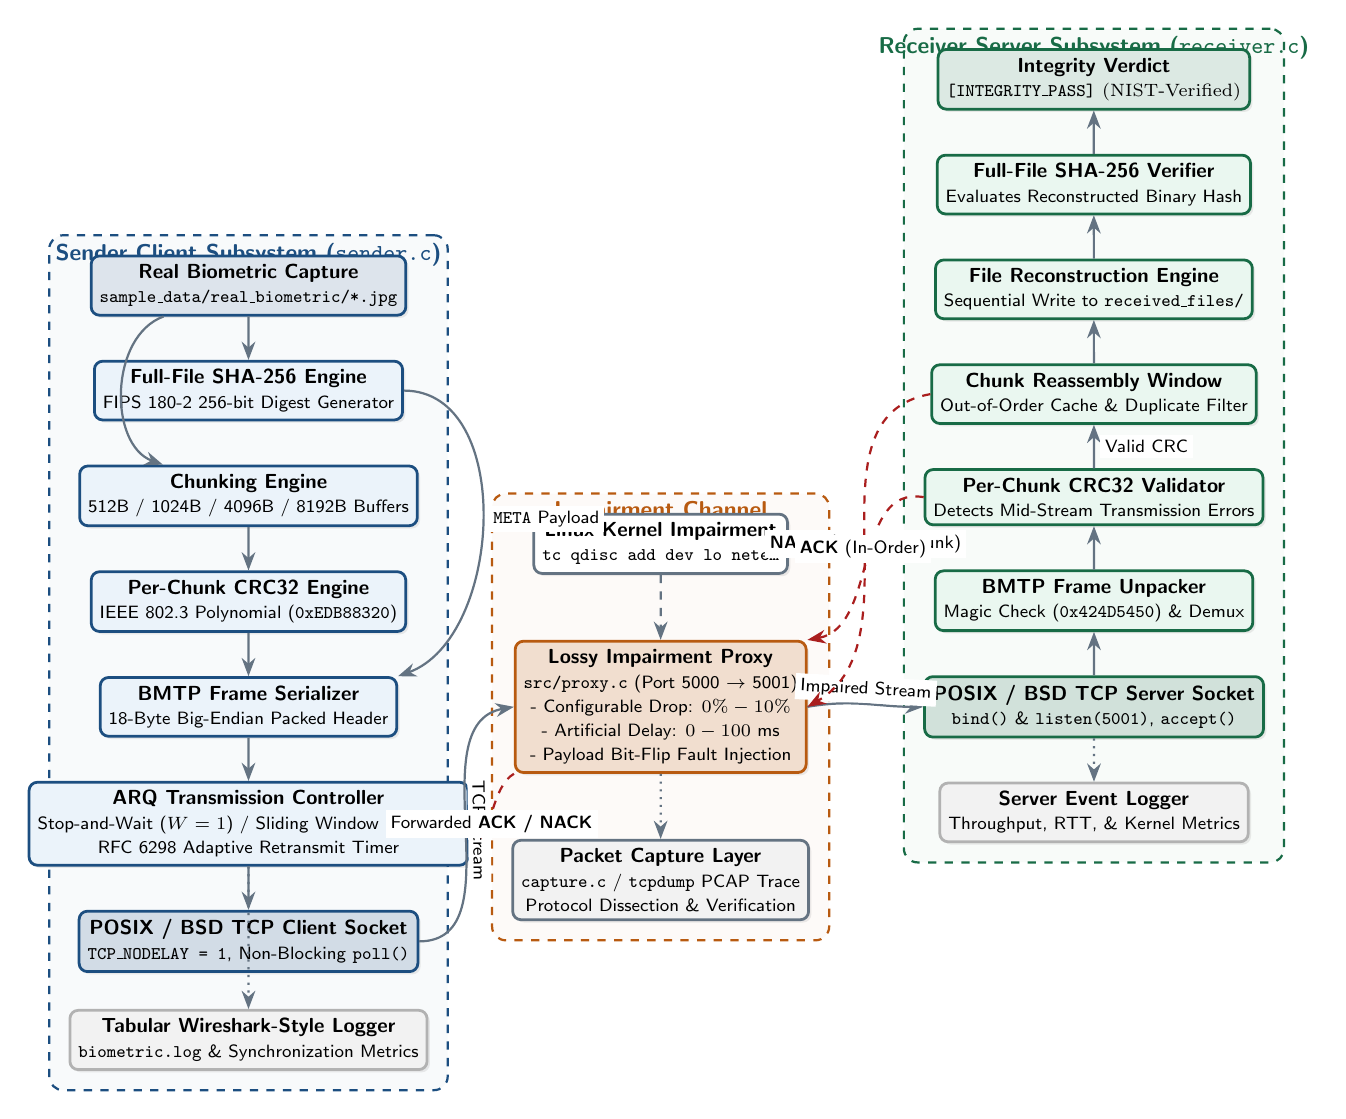
\begin{tikzpicture}[
    scale=0.92,
    every node/.style={transform shape},
    font=\sffamily\footnotesize,
    >=Stealth,
    node distance=0.8cm and 0.9cm,
    % Box styles
    senderbox/.style={
        rectangle, rounded corners=3pt,
        draw=senderblue, line width=1pt,
        fill=senderlight, text=black,
        align=center, minimum width=4.0cm, minimum height=0.75cm,
        drop shadow={opacity=0.15, shadow xshift=1pt, shadow yshift=-1pt}
    },
    receiverbox/.style={
        rectangle, rounded corners=3pt,
        draw=receivergreen, line width=1pt,
        fill=receiverlight, text=black,
        align=center, minimum width=4.0cm, minimum height=0.75cm,
        drop shadow={opacity=0.15, shadow xshift=1pt, shadow yshift=-1pt}
    },
    proxybox/.style={
        rectangle, rounded corners=3pt,
        draw=proxyorange, line width=1pt,
        fill=proxylight, text=black,
        align=center, minimum width=3.4cm, minimum height=0.75cm,
        drop shadow={opacity=0.15, shadow xshift=1pt, shadow yshift=-1pt}
    },
    subgroupbox/.style={
        rectangle, rounded corners=5pt,
        draw=#1, dashed, line width=0.8pt,
        inner sep=7pt
    },
    flowline/.style={
        ->, thick, draw=slateborder
    },
    feedbackline/.style={
        ->, thick, draw=accentcrimson, dashed
    },
    edgelabel/.style={
        fill=white, inner sep=2pt, font=\scriptsize\sffamily, text=black
    }
]

    % -------------------------------------------------------------
    % COLUMN 1: SENDER (CLIENT)
    % -------------------------------------------------------------
    \node[senderbox, fill=senderblue!15, font=\bfseries\sffamily\footnotesize] (s_file) {
        Real Biometric Capture\\
        \scriptsize\normalfont\texttt{sample\_data/real\_biometric/*.jpg}
    };

    \node[senderbox, below=0.6cm of s_file] (s_sha) {
        \textbf{Full-File SHA-256 Engine}\\
        \scriptsize FIPS 180-2 256-bit Digest Generator
    };

    \node[senderbox, below=0.6cm of s_sha] (s_chunk) {
        \textbf{Chunking Engine}\\
        \scriptsize 512B / 1024B / 4096B / 8192B Buffers
    };

    \node[senderbox, below=0.6cm of s_chunk] (s_crc) {
        \textbf{Per-Chunk CRC32 Engine}\\
        \scriptsize IEEE 802.3 Polynomial (\texttt{0xEDB88320})
    };

    \node[senderbox, below=0.6cm of s_crc] (s_proto) {
        \textbf{BMTP Frame Serializer}\\
        \scriptsize 18-Byte Big-Endian Packed Header
    };

    \node[senderbox, below=0.6cm of s_proto] (s_arq) {
        \textbf{ARQ Transmission Controller}\\
        \scriptsize Stop-and-Wait ($W=1$) / Sliding Window ($W>1$)\\
        \scriptsize RFC 6298 Adaptive Retransmit Timer
    };

    \node[senderbox, fill=senderblue!20, below=0.6cm of s_arq] (s_sock) {
        \textbf{POSIX / BSD TCP Client Socket}\\
        \scriptsize \texttt{TCP\_NODELAY = 1}, Non-Blocking \texttt{poll()}
    };

    \node[senderbox, fill=gray!10, draw=gray!60, below=0.5cm of s_sock] (s_log) {
        \textbf{Tabular Wireshark-Style Logger}\\
        \scriptsize \texttt{biometric.log} \& Synchronization Metrics
    };

    % -------------------------------------------------------------
    % COLUMN 2: NETWORK & IMPAIRMENT MIDDLEBOX
    % -------------------------------------------------------------
    \node[proxybox, fill=proxyorange!20, right=1.6cm of s_proto] (p_proxy) {
        \textbf{Lossy Impairment Proxy}\\
        \scriptsize \texttt{src/proxy.c} (Port 5000 $\to$ 5001)\\
        \scriptsize - Configurable Drop: $0\% - 10\%$\\
        \scriptsize - Artificial Delay: $0 - 100\text{ ms}$\\
        \scriptsize - Payload Bit-Flip Fault Injection
    };

    \node[proxybox, fill=white, draw=slateborder, above=0.9cm of p_proxy] (p_netem) {
        \textbf{Linux Kernel Impairment}\\
        \scriptsize \texttt{tc qdisc add dev lo netem}
    };

    \node[proxybox, fill=gray!10, draw=slateborder, below=0.9cm of p_proxy] (p_pcap) {
        \textbf{Packet Capture Layer}\\
        \scriptsize \texttt{capture.c} / \texttt{tcpdump} PCAP Trace\\
        \scriptsize Protocol Dissection \& Verification
    };

    % -------------------------------------------------------------
    % COLUMN 3: RECEIVER (SERVER)
    % -------------------------------------------------------------
    \node[receiverbox, fill=receivergreen!20, right=1.6cm of p_proxy] (r_sock) {
        \textbf{POSIX / BSD TCP Server Socket}\\
        \scriptsize \texttt{bind()} \& \texttt{listen(5001)}, \texttt{accept()}
    };

    \node[receiverbox, above=0.6cm of r_sock] (r_unpack) {
        \textbf{BMTP Frame Unpacker}\\
        \scriptsize Magic Check (\texttt{0x424D5450}) \& Demux
    };

    \node[receiverbox, above=0.6cm of r_unpack] (r_crc) {
        \textbf{Per-Chunk CRC32 Validator}\\
        \scriptsize Detects Mid-Stream Transmission Errors
    };

    \node[receiverbox, above=0.6cm of r_crc] (r_buf) {
        \textbf{Chunk Reassembly Window}\\
        \scriptsize Out-of-Order Cache \& Duplicate Filter
    };

    \node[receiverbox, above=0.6cm of r_buf] (r_recon) {
        \textbf{File Reconstruction Engine}\\
        \scriptsize Sequential Write to \texttt{received\_files/}
    };

    \node[receiverbox, above=0.6cm of r_recon] (r_sha) {
        \textbf{Full-File SHA-256 Verifier}\\
        \scriptsize Evaluates Reconstructed Binary Hash
    };

    \node[receiverbox, fill=receivergreen!15, font=\bfseries\sffamily\footnotesize, above=0.6cm of r_sha] (r_status) {
        Integrity Verdict\\
        \scriptsize\normalfont\texttt{[INTEGRITY\_PASS]} (NIST-Verified)
    };

    \node[receiverbox, fill=gray!10, draw=gray!60, below=0.6cm of r_sock] (r_log) {
        \textbf{Server Event Logger}\\
        \scriptsize Throughput, RTT, \& Kernel Metrics
    };

    % -------------------------------------------------------------
    % BACKGROUND GROUPING FRAMES
    % -------------------------------------------------------------
    \begin{scope}[on background layer]
        % Sender Subsystem Frame
        \node[subgroupbox=senderblue, fill=senderblue!3,
              fit=(s_file) (s_sock) (s_log),
              label={[anchor=north, text=senderblue, font=\bfseries\sffamily\small]north:\textbf{Sender Client Subsystem (\texttt{sender.c})}}] (sender_group) {};

        % Impairment Subsystem Frame
        \node[subgroupbox=proxyorange, fill=proxyorange!3,
              fit=(p_netem) (p_proxy) (p_pcap),
              label={[anchor=north, text=proxyorange, font=\bfseries\sffamily\small]north:\textbf{Impairment Channel}}] (proxy_group) {};

        % Receiver Subsystem Frame
        \node[subgroupbox=receivergreen, fill=receivergreen!3,
              fit=(r_status) (r_sock) (r_log),
              label={[anchor=north, text=receivergreen, font=\bfseries\sffamily\small]north:\textbf{Receiver Server Subsystem (\texttt{receiver.c})}}] (receiver_group) {};
    \end{scope}

    % -------------------------------------------------------------
    % ARROWS AND DATA FLOW PATHS
    % -------------------------------------------------------------
    % Sender internal
    \draw[flowline] (s_file) -- (s_sha);
    \draw[flowline] (s_file) to[out=200, in=160] (s_chunk);
    \draw[flowline] (s_chunk) -- (s_crc);
    \draw[flowline] (s_crc) -- (s_proto);
    \draw[flowline] (s_sha.east) to[out=0, in=20] node[edgelabel, right=2pt] {\texttt{META} Payload} (s_proto.north east);
    \draw[flowline] (s_proto) -- (s_arq);
    \draw[flowline] (s_arq) -- (s_sock);
    \draw[flowline, dotted] (s_arq) -- (s_log);

    % Channel Interconnections
    \draw[flowline] (s_sock.east) to[out=0, in=190] node[edgelabel, above, sloped] {TCP Stream} (p_proxy.west);
    \draw[flowline] (p_proxy.east) to[out=10, in=180] node[edgelabel, above, sloped] {Impaired Stream} (r_sock.west);
    \draw[flowline, dashed] (p_netem) -- (p_proxy);
    \draw[flowline, dotted] (p_proxy) -- (p_pcap);

    % Receiver internal
    \draw[flowline] (r_sock) -- (r_unpack);
    \draw[flowline] (r_unpack) -- (r_crc);
    \draw[flowline] (r_crc) -- node[edgelabel, right=2pt] {Valid CRC} (r_buf);
    \draw[flowline] (r_buf) -- (r_recon);
    \draw[flowline] (r_recon) -- (r_sha);
    \draw[flowline] (r_sha) -- (r_status);
    \draw[flowline, dotted] (r_sock) -- (r_log);

    % Feedback Loop: NACK and ACK from Receiver to Sender
    \draw[feedbackline] (r_crc.west) to[out=170, in=10] node[edgelabel, above] {\textbf{NACK} (Corrupt Chunk)} (p_proxy.north east);
    \draw[feedbackline] (r_buf.west) to[out=190, in=30] node[edgelabel, below] {\textbf{ACK} (In-Order)} (p_proxy.east);
    \draw[feedbackline] (p_proxy.south west) to[out=210, in=330] node[edgelabel, below] {Forwarded \textbf{ACK / NACK}} (s_arq.east);

\end{tikzpicture}
\caption{BMTP End-to-End System Architecture showcasing functional blocks, cryptographic verification layers, and ARQ feedback loops.}
\label{fig:arch}
\end{figure}

\vspace{1em}

% =========================================================================
% SECTION 2: BINARY PROTOCOL FRAMING
% =========================================================================
\section{Application-Layer Binary Framing (BMTP Header)}

TCP provides a continuous, unstructured byte stream. To enforce strict application message boundaries and prevent buffer overrun vulnerabilities, every BMTP Protocol Data Unit (PDU) starts with an explicit, 18-byte packed binary header encoded in Big-Endian network byte order.

\begin{figure}[htbp]
\centering
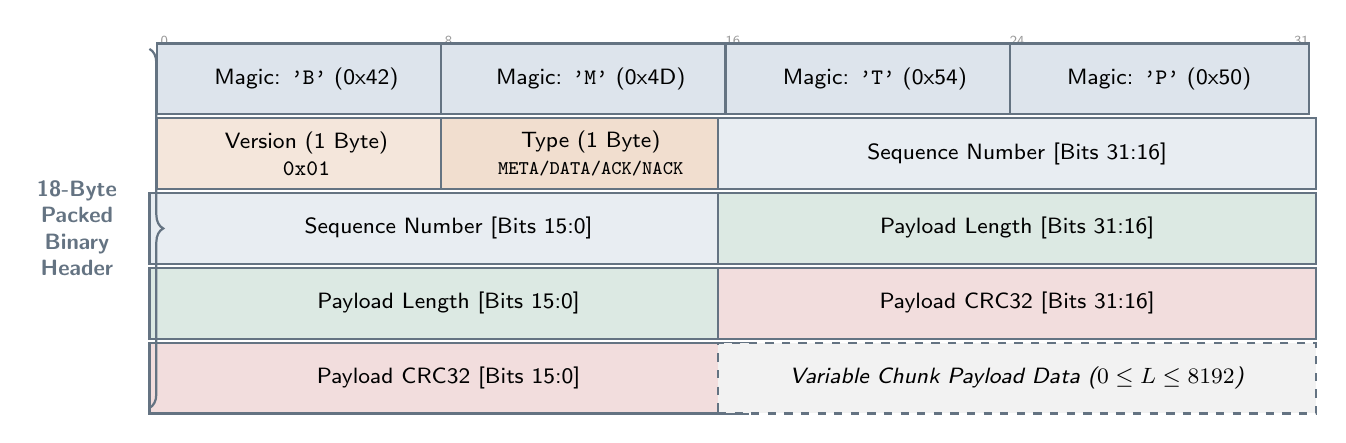
\begin{tikzpicture}[
    scale=0.95,
    font=\sffamily\footnotesize,
    box/.style={
        draw=slateborder, line width=0.8pt, fill=headerfill,
        minimum height=0.9cm, align=center
    },
    bitnode/.style={
        font=\tiny\sffamily, text=gray!80
    }
]

    % Bit Index Indicators
    \foreach \i/\b in {0/0, 4/8, 8/16, 12/24, 16/31} {
        \node[bitnode] at (\i*0.95, 0.5) {\b};
    }

    % Row 0: Bytes 0-3 (Magic 0x424D5450)
    \node[box, fill=senderblue!15, minimum width=3.8cm] at (1.9, 0) {Magic: \texttt{'B'} (0x42)};
    \node[box, fill=senderblue!15, minimum width=3.8cm] at (5.7, 0) {Magic: \texttt{'M'} (0x4D)};
    \node[box, fill=senderblue!15, minimum width=3.8cm] at (9.5, 0) {Magic: \texttt{'T'} (0x54)};
    \node[box, fill=senderblue!15, minimum width=3.8cm] at (13.3, 0) {Magic: \texttt{'P'} (0x50)};

    % Row 1: Bytes 4-7 (Version, Type, High 16-bits of Seq)
    \node[box, fill=proxyorange!15, minimum width=3.8cm] at (1.9, -1.0) {Version (1 Byte)\\ \texttt{0x01}};
    \node[box, fill=proxyorange!20, minimum width=3.8cm] at (5.7, -1.0) {Type (1 Byte)\\ \scriptsize\texttt{META/DATA/ACK/NACK}};
    \node[box, fill=senderblue!10, minimum width=7.6cm] at (11.4, -1.0) {Sequence Number [Bits 31:16]};

    % Row 2: Bytes 8-11 (Low 16-bits of Seq, High 16-bits of Payload Len)
    \node[box, fill=senderblue!10, minimum width=7.6cm] at (3.8, -2.0) {Sequence Number [Bits 15:0]};
    \node[box, fill=receivergreen!15, minimum width=7.6cm] at (11.4, -2.0) {Payload Length [Bits 31:16]};

    % Row 3: Bytes 12-15 (Low 16-bits of Payload Len, High 16-bits of CRC32)
    \node[box, fill=receivergreen!15, minimum width=7.6cm] at (3.8, -3.0) {Payload Length [Bits 15:0]};
    \node[box, fill=accentcrimson!15, minimum width=7.6cm] at (11.4, -3.0) {Payload CRC32 [Bits 31:16]};

    % Row 4: Bytes 16-17 + Variable Payload
    \node[box, fill=accentcrimson!15, minimum width=7.6cm] at (3.8, -4.0) {Payload CRC32 [Bits 15:0]};
    \node[box, fill=gray!10, dashed, minimum width=7.6cm] at (11.4, -4.0) {\textit{Variable Chunk Payload Data ($0 \le L \le 8192$)}};

    % Annotations
    \draw[decorate, decoration={brace, amplitude=5pt}, thick, slateborder]
        (-0.2, 0.4) -- (-0.2, -4.4)
        node[midway, left=8pt, font=\sffamily\footnotesize\bfseries, align=center] {
            18-Byte\\Packed\\Binary\\Header
        };

\end{tikzpicture}
\caption{Bitwise layout of the packed 18-byte BMTP PDU header structure.}
\label{fig:header}
\end{figure}

\begin{table}[htbp]
\centering
\small
\begin{tabular}{@{}llcp{7.8cm}@{}}
\toprule
\textbf{Field Name} & \textbf{C Datatype} & \textbf{Bytes} & \textbf{Description \& Framing Purpose} \\
\midrule
\texttt{magic} & \texttt{uint8\_t[4]} & 4 & Synchronization constant \texttt{0x424D5450} (\texttt{"BMTP"}). Mismatches trigger immediate connection reset. \\
\texttt{version} & \texttt{uint8\_t} & 1 & Protocol revision marker (\texttt{0x01}). \\
\texttt{msg\_type} & \texttt{uint8\_t} & 1 & Operational opcode: \texttt{1:META}, \texttt{2:DATA}, \texttt{3:ACK}, \texttt{4:NACK}, \texttt{5:END}, \texttt{6:ERROR}. \\
\texttt{seq\_num} & \texttt{uint32\_t} & 4 & Big-endian monotonically increasing sequence identifier ($0 \le seq < \text{total\_chunks}$). \\
\texttt{payload\_len} & \texttt{uint32\_t} & 4 & Explicit payload length in bytes. Bounds receive buffers against overflow. \\
\texttt{crc32} & \texttt{uint32\_t} & 4 & IEEE 802.3 32-bit checksum computed over the chunk payload (\texttt{0xEDB88320}). \\
\bottomrule
\end{tabular}
\caption{Detailed field specification of the BMTP binary framing header.}
\label{tab:header_fields}
\end{table}

% =========================================================================
% SECTION 3: SEQUENCE & PROTOCOL LIFECYCLE
% =========================================================================
\section{Protocol Lifecycle \& ARQ Retransmission Sequence}

Figure~\ref{fig:seq} illustrates the complete session workflow, including connection setup, the initial cryptographic metadata exchange, Stop-and-Wait/Sliding Window chunk delivery, dynamic NACK-triggered fast retransmission, and final end-to-end SHA-256 integrity validation.

\begin{figure}[htbp]
\centering
\begin{tikzpicture}[
    scale=0.92,
    every node/.style={transform shape},
    font=\sffamily\footnotesize,
    >=Stealth,
    lifeline/.style={thick, draw=slateborder, dashed},
    eventnode/.style={fill=white, draw=slateborder, rounded corners=2pt, font=\scriptsize\sffamily, align=center, inner sep=3pt},
    msg/.style={->, thick, draw=senderblue},
    ackmsg/.style={<-, thick, draw=receivergreen},
    failmsg/.style={->, thick, draw=accentcrimson},
    notebox/.style={fill=gray!10, draw=slateborder, rounded corners=3pt, font=\scriptsize\sffamily, align=center, inner sep=4pt}
]

    % Lifeline entities
    \node[senderbox, minimum width=3.2cm] (send) at (0, 0) {\textbf{Sender Client}};
    \node[proxybox, minimum width=3.2cm] (chan) at (6.0, 0) {\textbf{Impairment Channel}};
    \node[receiverbox, minimum width=3.2cm] (recv) at (12.0, 0) {\textbf{Receiver Server}};

    \draw[lifeline] (send.south) -- (0, -12.5);
    \draw[lifeline] (chan.south) -- (6.0, -12.5);
    \draw[lifeline] (recv.south) -- (12.0, -12.5);

    % Phase 1: TCP Handshake
    \node[notebox, minimum width=13cm] at (6.0, -0.8) {\textbf{Phase 1: TCP Handshake \& Socket Tuning} (\texttt{TCP\_NODELAY = 1})};
    \draw[msg] (0, -1.3) -- node[above, font=\scriptsize] {\texttt{TCP SYN}} (6.0, -1.5);
    \draw[msg] (6.0, -1.5) -- (12.0, -1.7);
    \draw[ackmsg] (6.0, -2.1) -- node[above, font=\scriptsize] {\texttt{TCP SYN-ACK}} (12.0, -1.9);
    \draw[ackmsg] (0, -2.3) -- (6.0, -2.1);
    \draw[msg] (0, -2.5) -- node[above, font=\scriptsize] {\texttt{TCP ACK} [Established]} (12.0, -2.9);

    % Phase 2: Metadata Exchange
    \node[notebox, minimum width=13cm] at (6.0, -3.5) {\textbf{Phase 2: Cryptographic Metadata Exchange}};
    \draw[msg] (0, -4.1) -- node[above, font=\scriptsize] {\texttt{BMTP [META]} (File Size, Total Chunks, Expected SHA-256)} (12.0, -4.5);
    \draw[ackmsg] (0, -5.1) -- node[above, font=\scriptsize] {\texttt{BMTP [ACK 0]}} (12.0, -4.7);

    % Phase 3: Data Transmission & ARQ Fast Retransmit
    \node[notebox, minimum width=13cm] at (6.0, -5.7) {\textbf{Phase 3: DATA PDU Streaming with Per-Chunk CRC32 \& NACK Fast Retransmission}};
    \draw[msg] (0, -6.3) -- node[above, font=\scriptsize] {\texttt{BMTP [DATA]} (Seq: 0, CRC32: \texttt{0x9A4F})} (12.0, -6.7);
    \draw[ackmsg] (0, -7.3) -- node[above, font=\scriptsize] {\texttt{BMTP [ACK 0]}} (12.0, -6.9);

    % Corrupted frame
    \draw[msg] (0, -7.8) -- node[above, font=\scriptsize] {\texttt{BMTP [DATA]} (Seq: 1, CRC32: \texttt{0x2C8E})} (6.0, -8.0);
    \node[eventnode, draw=accentcrimson, text=accentcrimson] at (6.0, -8.3) {Fault Injection: Bit-Flip in Payload};
    \draw[failmsg] (6.0, -8.6) -- node[above, font=\scriptsize] {Corrupted PDU} (12.0, -8.8);
    \node[eventnode, draw=accentcrimson, text=accentcrimson] at (12.0, -9.1) {CRC Check Mismatch!};
    
    % NACK Fast Retransmit
    \draw[ackmsg, draw=accentcrimson] (6.0, -9.6) -- node[above, font=\scriptsize, text=accentcrimson] {\texttt{BMTP [NACK 1]} (Fast Retransmit Request)} (12.0, -9.4);
    \draw[ackmsg, draw=accentcrimson] (0, -9.8) -- (6.0, -9.6);

    \draw[msg] (0, -10.3) -- node[above, font=\scriptsize] {\texttt{BMTP [DATA]} (Seq: 1, Retransmit Uncorrupted)} (12.0, -10.7);
    \draw[ackmsg] (0, -11.3) -- node[above, font=\scriptsize] {\texttt{BMTP [ACK 1]}} (12.0, -10.9);

    % Phase 4: Verification and Teardown
    \node[notebox, minimum width=13cm] at (6.0, -11.8) {\textbf{Phase 4: END Frame, Full-File SHA-256 Attestation, and Graceful FIN Teardown}};
    
\end{tikzpicture}
\caption{BMTP execution trace showcasing the 4-phase transaction lifecycle.}
\label{fig:seq}
\end{figure}

% =========================================================================
% SECTION 4: ARCHITECTURAL DESIGN HIGHLIGHTS
% =========================================================================
\section{Architectural Rationale \& Transport Analysis}

\begin{enumerate}
    \item \textbf{Decoupled Dual-Tier Integrity}: By segregating transmission-level verification (per-chunk IEEE 802.3 CRC32) from storage-level attestation (full-file FIPS 180-2 SHA-256), individual corrupted chunks are recovered instantaneously without requiring entire biometric file retransmissions.
    \item \textbf{Explicit Frame Boundary Delineation}: Standard TCP stream sockets concatenate writes. The fixed 18-byte packed header guarantees deterministic parsing and immediate detection of desynchronized sockets via the \texttt{BMTP} magic constant.
    \item \textbf{Zero Buffer Overflow Footprint}: Dynamic chunk buffers allocate memory strictly bound to \texttt{payload\_len}, fully resisting malicious framing overruns.
\end{enumerate}

\end{document}
